\documentclass[14pt, a4paper]{extreport} % или article, если не нужен увеличенный базовый шрифт
\usepackage[utf8]{inputenc}
\usepackage[T2A]{fontenc}
\usepackage[russian]{babel}
\usepackage{array}
\usepackage{graphicx}
\usepackage{ulem}
\usepackage{geometry}
\geometry{top=2cm, bottom=2cm, left=2cm, right=2cm}
\usepackage{tabularx}
\usepackage{amsmath}
\usepackage{amssymb}
\usepackage{multirow}
\usepackage{booktabs}
\usepackage{float}
\usepackage{tabularx}
\usepackage{booktabs}
\usepackage{siunitx}
\usepackage{indentfirst}
\usepackage{placeins}
\usepackage{lipsum}
\usepackage{longtable}
\usepackage{csquotes}
\usepackage[style=gost-numeric,sorting=none]{biblatex}
\usepackage{enumitem}
\usepackage{caption}
\usepackage{subfiles}
\captionsetup[table]{position=top, singlelinecheck=false, justification=raggedleft}
\usepackage{wrapfig}
\usepackage{setspace}
\usepackage{totpages}
\usepackage{ifthen}
\usepackage{refcount}

\usepackage{tabto}

\addbibresource{references.bib}
\usepackage{titlesec}
\titleformat{\chapter}[display]
    {\normalfont\huge\bfseries}
    {\chaptertitlename\ \thechapter}
    {20pt}
    {\Huge}
\usepackage{booktabs}
\usepackage{makecell}
\graphicspath{{Image/}}

\geometry{
    a4paper,
    total={170mm,257mm},
    left=20mm,
    top=20mm,
}

\newcommand{\specialcell}[2][c]{%
    \begin{tabular}[#1]{@{}c@{}}#2\end{tabular}%
}

\usepackage{etoolbox}
\patchcmd{\thebibliography}
  {\chapter*{\bibname}}
  {\section*{\centering СПИСОК ЛИТЕРАТУРЫ}}
  {}{}
\patchcmd{\thebibliography}
  {\addcontentsline{toc}{chapter}{\bibname}}
  {\addcontentsline{toc}{section}{СПИСОК ЛИТЕРАТУРЫ}}
  {}{}


\usepackage{setspace}
\onehalfspacing


% Для подчеркивания текста, аналогичного .underline в Word
\newcommand{\und}[1]{\uline{#1}}

\begin{document}

\subfile{titul.tex}

\newpage
\tableofcontents

\newpage
\section*{Введение}
Данная курсовая работа посвящена нахождению оптимальных параметров артиллерийского орудия и условий заряжания путем решения обратной задачи внутреннй баллистики.
Ключевым критерием оптимальности решения является критерий качества баллистического решения $Z_{\text{B1}}$. 

Решение должно удовлетворять следующим требованиям: 
\begin{itemize}
    \item  $p_{\text{m}}^{\text{max}}$ $\leq$ 390 МПа
    \item $l_{\text{m}}^{\text{max}}$ $\leq$ 65 ед.d
\end{itemize}

Также на решение наложены следующие ограничения: 
\begin{itemize}
    \item  $v_{\text{pm-50}}$ = 830 $\text{м/c}$
    \item $p_{\text{mz+50}}$ = 180 МПа
\end{itemize}

Условие задания: 
\begin{itemize}
    \item $d$ = 85 мм
    \item $q$ = 5 кг
    \item $v_{\text{pm}}$ = 950 $\text{м/c}$
    \item Тип орудения -- нарезное (НР)
    \item Тип мат. модели -- квазиодномерная (КМ)
\end{itemize}

Данная задача будет решаться с использованием мат. аппарата квазиодномерной модели внутренней.
баллистики. Также использованы методы оптимизации для нахождения оптимального решения обратной задачи с учетом критериев и ограничений.

Вычисления проводились с помощью языка программирования Python с использованием библиотеки PyBallistics [1], визуализация данных осуществлялась 
через библиотеку Matplotlib [2].

\newpage
\chapter{Прямая задача внутренней баллистики}
\section{Описание математической модели}

Выстрел предствавляет собой довольно сложный быстропротекающий физико-химический процесс. Его физическая сущность состоит в том, что при сгорании порохового заряда образуются газообразные продукты сгорания под большим давлением, 
под действием которого снаряд выталкивается из канала ствола с огромной скоростью. Прямая задача состоит в том, чтобы описать движение снаряда массой $q$ по каналу ствола диаметра $d$ под действием давления продуктов сгорания заряда пороха массой $\omega$, находящимся в объеме $W_0$. Схема процесса вместе с качественными распределениями давления и скорости представлена на рисунке 1.
Для упрощения вводится ствол с камерой приведенной длины $l_0$, имеющей тот же обеъем $W_0$, но с диаметром, равным калибру ствола $d$. Схема упрощения представлена на рисунке 1.2. 

\begin{figure}[h!]
\centering

\includegraphics[width=0.45\textheight]{imgs/1.jpg}
\caption{Схема процесса выстрела}
\end{figure}

\begin{figure}[h]
\centering
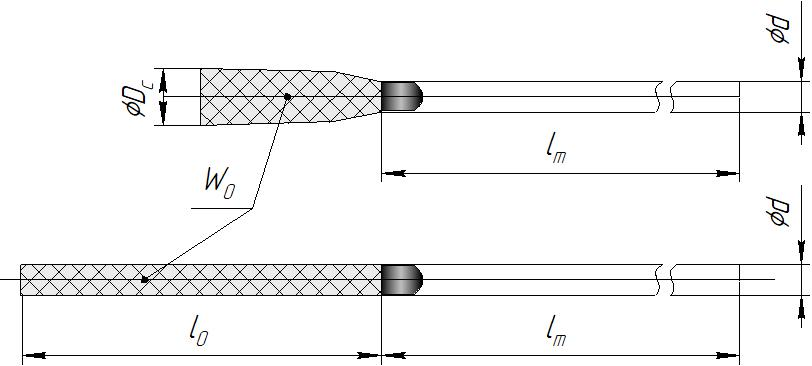
\includegraphics[width=0.5\textheight]{imgs/2.jpg}
\caption{Схема упрощения}
\end{figure}

Наиболее соверменным и точным описанием процесса выстрела является газодинамический подход, 
по размерности в нашем случае модель является одномерной (квазиодномерной). Эта модель выстрела содержит некоторые допущения: 
\begin{itemize}
    \item Гипотеза односкоростной газопороховой смеси (ОГПС)
    \item Геометрический закон горения пороха
\end{itemize}


    В пространстве между дном ствола и дном снаряда (заснарядный объём) в процессе движения снаряда 
по каналу ствола находятся газообразные продукты сгорания пороха и конденсированные частицы несгоревшего пороха.
Для упрощения принимается, что пороховые газы и конденсированные элементы представляют собой гомогенную смесь, которая движется 
с общей скоростью. Такое допущение называется гипотезой односкоростной газопороховой смеси (ОГПС). Уравнение состояния ОГПС представляется в виде: 

\begin{equation}
\varepsilon = \frac{p}{k - 1} \left( \frac{1}{\rho} - \frac{1 - \psi}{\delta} - b \psi \right) + (1 - \psi) \frac{f}{k - 1},
\label{eq:epsilon}
\end{equation}
где $\varepsilon$ -- удельная внутрення энергия ОГПС, $\rho$ -- плотность ОГПС, $b$ -- коволюм порохового газа (эффективный собственный объём молекул), $k$ -- показатель адиабаты, 
$\psi$ = $\omega_b$ / $\omega$ -- отношение массы сгоревшего элемента у его исходной массе, $\omega_b$ -- масса сгоревшего пороха, $\omega$ -- исходная масса пороха. $\delta$ -- плотность пороха. 

Геометрический закон горения пороха выражается в виде формулы (1.2): 

\begin{equation}
\frac{dz}{dt} = \frac{p^\nu}{I_e}, 
\label{eq:1}
\end{equation}
где  $p$ -- давление газа, $\nu$ -- показатель степени
в законе горения. В артиллерии, как правило, $\nu$ = 1. $z$ = $e$ /$e_1$ -- безразмерная толщина сгоревшего свода порохового элемента. В свою очередь
$e$ -- координата текущего положения поверхности горения, а $e_1$ -- полная толщина горящего свода порохового элемента. $I_e$ -- полный импульс давления пороховых газов:
\[
I_e = \int_0^{t_e} p^v  dt = \frac{e_1}{u_1},
\]

где $u_1$ -- скорость горения при единичном горении, определяемая экспериментальным путем.

Далее рассмотрим систему уравнений для газодинамической задачи в приближении ОГПС. ОГПС в данном случае представляет собой «псевдогаз», её движение в заснарядном
объёме описывается стандартными уравнениями сохранения массы, импульса и энергии в лагранжевых координатах: 

\begin{equation}
\frac{\partial v}{\partial m} = \frac{d}{dt}\left(\frac{1}{\rho S}\right)
\end{equation}

\begin{equation}
\frac{dv}{dt} + S\frac{\partial p}{\partial m} = 0,
\end{equation}

\begin{equation}
\frac{d\epsilon}{dt} + p\frac{\partial}{\partial m}(vS) = 0.
\end{equation}

Здесь $m$ -- массовая лагранжева координата.

Для математического описания процесса выстрела необходимо установить закономерность газообразования, то есть связь между геометрическими размерами порохового элемента (ПЭ) и количеством пороховых газов (ПГ), образованных в процессе выгорания заряда, а также интенсивностью их образования. Такую зависимость называют функцией газоприхода $\psi(z)$:

\begin{equation}
\psi(z) = \kappa z (1 + \lambda z + \mu z^2),
\end{equation}

где $k, \lambda, \mu$ -- коэффиценты формы порохового зерна (порохового элемента).
На практике для расчётов пользуются упрощенной формой записи данного закона:

\begin{equation}
\psi(z) = \kappa z (1 + \lambda z),
\end{equation}
где коэффицинты $k, \lambda$ определяются путём приравнивания функций $\psi$, полученных расчётом по формулам (1.6) и (1.7) в точках $z$ = 0.5 и $z$ = 1.

Чтобы замкнуть систему уравнений, необходимо записать уравнение движения снаряда по каналу ствола:

\begin{equation}
q \, \frac{d v_{p}}{d t} = S p_{p} - R,
\end{equation}
где $q$-- масса снаряда, $v_p$ -- скорость скорость снаряда, $S$-- площадь поперечного сечения канала ствола, $ p_{p}$ -- давление на дно снаряда, $R$ -- суммарная сила сопротивлению движения снаряда. 

Запишем теперь полученную систему уравнений: 

\[
\left\{
\begin{array}{l}
\dfrac{\partial v}{\partial m} = \dfrac{d}{dt}\left(\dfrac{1}{\rho S}\right) \\[1.5ex]
\dfrac{dv}{dt} + S\dfrac{\partial p}{\partial m} = 0 \\[1.5ex]
\dfrac{d\varepsilon}{dt} + p\dfrac{\partial}{\partial m}(vS) = 0 \\[1.5ex]
\varepsilon = \dfrac{p}{k - 1} \left( \dfrac{1}{\rho} - \dfrac{1 - \psi}{\delta} - b \psi \right) + (1 - \psi) \dfrac{f}{k - 1} \\[1.5ex]
\dfrac{dz}{dt} = \dfrac{p^\nu}{I_e} \\[1.5ex]
q \, \dfrac{d v_{p}}{d t} = S p_{p} - R
\end{array}
\right.
\]

В дальнейшем данная система уравнений будет преобразовываться, так что это не конечный вид.

\section{Сила сопротивления движению снаряда по каналу ствола}

В процессе выстрела на снаряд действует не только сила давления пороховых газов, но и сила врезания ведущих поясков снаряда в нарезы, сила трения ведущих устройств о поверхность нарезов и сила сопротивления сжатию столба воздуха перед снарядом. 

Начальный этап движения снаряда включает в себя врезание ведущих поисков в нарезы. Это весьма сложный процесс, в котором необходимо учитывать пластичекую деформацию медного пояска снаряда. В расчетах применяется гипотеза мнгновенного врезания: движения снаряда начинается тогда, когда давление на дно снаряда достигает 
некоторого условного предела, называемого давлением форсирования $p_0$. Для разных типов орудий значение данного предела может отличаться. Так, для нарезных стволов и снарядов с одним ведущим поясков $p_0$ = 30 МПа, что соответсвует данному варианту курсовой работы.

Классическим решением учета большей части форм сопротивления является домножение массы снаряда на некоторый коэффициент фиктивности $\phi$.

Рассмотрим две наибольшие состовляющие сил сопротивления движению снаряда -- сила, возникающая при сжатии столба воздуха во время движения снаряда и сила сопротивления движения по нарезам. Тогда суммарная сила сопротивления
движению снаряда представляет: 

\begin{equation}
R = p_a S + R_b,
\end{equation}
где $p_a$ -- давление воздушного столба перед снарядом, $R_b$ -- сила взаимодействия ведущих устройств (нарезов)
со снарядом.

Противодействие воздуха перед снарядом имеет сущесвтенное влияние, которое необходимо учитывать. Особенно это проявляется при движении снаряда 
со сверхзвуковой скоростью относительно невозмущенного воздуха. Данный фактор можно приближеннго учесть с помощью известной зависимости для точного решения задачи о поршне, сжимающем газ:

\begin{equation}
P_a = P_{0a} \left(1 + \frac{k_a(k_a+1)}{4} \left(\frac{\upsilon_p}{c_{0a}}\right)^2 + 
k_a \frac{\upsilon_p}{c_{0a}} \sqrt{1 + \left(\frac{k_a+1}{4} \frac{\upsilon_p}{c_{0a}}\right)^2} \right),
\end{equation}
где $k_a$, $P_{0a}$ и $c_{0a}$ — показатель адиабаты, давление и скорость звука в невозмущённом воздухе.

Для учёта силы трения в нарезах используется данная формула коэффициента фиктивной массы снаряда: 

\begin{equation}
\varphi = \varphi_1 + \frac{\omega}{3q}.
\label{eq:phi_equation}
\end{equation}
где $\varphi_1 \approx$  1.02.

\section{Учёт потерь на теплоотдачу в стенки ствола}

Основым источником теплопотерь при выстреле является теплоотдача в стенки ствола. Интенсивность этого процесса определяется разностью температур раскалённых пороховых газов и холодной стенки ствола. Ниже представлен упрощённый расчёт, который применим и к газодинамической модели.
Рассмотрим основное уравнение внутренней баллистики с учётом тепловых потерь:

\begin{equation}
\frac{k-1}{2} \varphi q v_p^2 = f \omega \psi - p_m \left( W_p - \frac{\omega}{\delta} + \left( \frac{1}{\delta} - b \right) \omega \psi \right) + p_{\text{ign}} \left( W_0 - \frac{\omega}{\delta} \right) - Q_w.
\end{equation}

В свою очередь, затраченная на теплоотдачу энергия может быть вычислена из следующих соображений:

\begin{equation}
\frac{dQ_{w}}{dt} = S_{w} q_{w},
\end{equation}

\begin{equation}
q_{w} = \mathrm{Nu} \frac{\lambda_g}{d} (T - T_{w}) = 0.023 \, \mathrm{Re}^{0.8} \, \mathrm{Pr}^{0.4} \frac{\lambda_g}{d} (T - T_{w}),
\end{equation}
где Nu -- число Нуссельта; Re -- число Рейнольдса; Pr -- число Прандтля (для порохового газа Pr = 0.74); $\lambda_g$ -- теплопроводность пороховых газов; $d$ -- диаметр канала (калибр); $S_w$ -- площадь поверхности теплоотдачи (площадь контакта пороховых газов со стволом).

Число Рейнольдса определяется по формуле:

\begin{equation}
\mathrm{Re} = \frac{\rho v d}{\mu},
\end{equation}
где $v$ -- средняя скорость потока; $\mu$ -- коэффициент динамической вязкости.
 
Средняя температура стенки \( T_w \) определяется по приближенной методике Р. Е. Соркина:

\begin{equation}
\frac{d\eta_T}{dt} = \frac{2 \mathrm{Nu}^2 \lambda_g^2}{d^2 c_b \rho_b \lambda_b} \left( T - T_0 - \sqrt{n_T} \right),
\end{equation}
где \( \sqrt{n_T} = T_w - T_0 \); \( n_T(0) = 0 \); \( c_b, \, \rho_b \) и \( \lambda_b \) — теплоёмкость, плотность и теплопроводность материала ствола соответственно; \( T_0 \) — начальная температура.

Коэффициент динамической вязкости пороховых газов может быть аппроксимирован формулой Сазерленда:

\begin{equation}
\mu = \mu_0 \mathrm{Pr} \frac{T_{cs} + T_{0s}}{T_{cs} + T} \left( \frac{T}{T_{0s}} \right)^{1.5},
\tag{1.43}
\end{equation}

где \( \mu_0 = 0.175 \cdot 10^{-4} \, \text{Па·с} \); \( T_{0s} = 273 \, \text{K} \); \( T_{cs} = 628 \, \text{K} \).

Площадь контакта \( S_w \) пороховых газов со стволом увеличивается по мере движения снаряда, причём увеличивается за счёт новой, «холодной» площади канала ствола. Вследствие этого средняя температура стенки \( T_w \) уменьшается.

Это можно учесть добавлением слагаемого \( v_n \) в формуле (1.42):

\begin{equation}
\frac{dn_T}{dt} = \frac{2 \mathrm{Nu}^2 \lambda_g^2}{d^2 c_b \rho_b \lambda_b} \left( T - T_0 - \sqrt{n_T} \right) + v_n.
\end{equation}

Выражение для \( v_\eta \) можно получить из следующих соображений: пусть в определённый момент времени средняя температура поверхности ствола за снарядом составляет \( T_w \). Снаряд движется со скоростью \( v_p \) и за время \( dt \) к площади теплоотдачи добавляется новая поверхность ствола с температурой \( T_{w0} \). При этом средняя температура ствола за время \( dt \) будет равна:

Отсюда можно определить \( v_n \):

\[
v_n = \lim_{dt \to 0} \frac{\eta_{T1} - \eta_T}{dt} = \lim_{dt \to 0} \frac{(T_{w1} - T_{w0})^2 - (T_w - T_{w0})^2}{dt} = -\frac{2v_p (T_w - T_{w0})^2}{x_p} = -\frac{2v_p \eta_T}{x_p}.
\]

Учёт теплоотдачи в стенки ствола в газодинамических моделях внутренней баллистики должен осуществляться совместно с решением пространственной задачи нагрева ствола. В большинстве случаев такая задача сопоставима по трудоёмкости с решением задачи внутренней
баллистики. При этом следует отметить, что в случае единичного выстрела учёт нагрева стенок ствола слабо влияет на основные баллистические характеристики. Поэтому, в ряде случаев можно считать температуру стенок ствола постоянной на протяжении выстрела [3].

Стоит отметить, что в случае квазиодномерной постановки расчёт теплоотдачи необходимо применть к каждой ячейке на расчётной сетке.

\section{Особенности расчёта смеси порохов}

Рассмотрим случай, когда пороховой заряд состоит из смеси порохов, которые могут характеризоватсья различными параметрами и формой порохового элемента. В данном случае продукты сгорания различных марок порохов образуют общую смесь газов.

Уравнение состояние ОГПС принимает следующий вид:

\begin{equation}
\varepsilon = \frac{1}{k-1} P_m \left[ \frac{1}{\rho} - \sum_{i=1}^N \frac{C_i (1 - \psi_i)}{\delta_i} - \sum_{i=1}^N C_i \psi_i b_i \right] + \sum_{i=1}^N C_i (1 - \psi_i) \frac{f_i}{k_i - 1}; 
\end{equation}

\begin{equation}
k = 1 + \frac{\sum_{i=1}^N C_i \psi_i R_{g,i}}{\sum_{i=1}^N \dfrac{C_i \psi_i R_{g,i}}{k_i - 1}}; \quad C_i = \frac{\omega_i}{\sum_{j=1}^N \omega_j},
\end{equation}
где \( C_i, \psi_i, \delta_i, b_i, f_i, k_i, R_{g,i}, \omega_i \) -- массовая доля пороховых газов, доля сгоревшего пороха, плотность пороха, коволюм порохового газа, сила пороха, показатель адиабаты, газовая постоянная пороховых газов и масса \(i\)-й навески смеси соответственно.

\section{Начальные и граничные условия}

При решении задач физики, описываемых дифференциальными уравнениями, как правило, известно и начальное состояние (положение) системы. В терминах теории дифференциальных уравнений такая информация называется начальными условиями. Отыскание частного решения дифференциального уравнения (системы уравнений) c использованем начальных условий (НУ) называется задачей Коши [4].
В контексте описания процесса выстрела постановка начальных условий зависит от момента времени, который принимается за начало отсчёта.
До момента форсирования снаряда (в
предположении о мгновенном воспламенении всего порохового заряда в
начальный момент) можно считать, что распределение всех параметров в
камере не зависит от координаты, поэтому процесс от момента воспламенения
до момента форсирования описывается всеми моделями одинаково [3].

В случае отсчета от момента вспышки, начальные условия имеют вид:

\begin{itemize}
    \item для ОГПС: \( v = 0; \, \rho = \Delta; \, p = p_{\text{ign}}; \, z = 0; \, \psi = 0. \)
    \item для снаряда: \( x_p = 0; \, v_p = 0. \)
\end{itemize}

В этом случае до достижения момента форсирования, определяемого условием \( p_m - p_a > p_0 \), снаряд должен оставаться неподвижным.

Здесь стоит уточнить смысл величины $p_{\text{ign}}$ -- давления вспышки. При сгорании воспламенительного заряда, который, как правило, состоит из дымного пороха с низким значением $I_e$, что позволяет получить в относительно короткое время около $10^5$ Па давления.

При решении задачи в газодинамической постановке помимо начальных условий требуется задать также и граничные условия. В качестве таковых выбираются условия непротекания (равенство скорости газа скорости поверхности) как на левой неподвижной границе (дно канала) расчетной области, так и на правой подвижной границе (дно снаряда) [3]:

\[
v(t, x = 0) = 0; \quad v(t, x = x_p) = v_p.
\]

При этом координата \( x_p \) -- переменная и отвечает текущему положению снаряда.

Влияние начальной температуры заряда на характеристики пороха учитывается путем пересчета силы пороха и импульса пороха:

\begin{equation}
I_e = I_e^{+20} \left[ 1 - K_I \left( T_0 - 293.15 \right) \right],
\end{equation}

\begin{equation}
f = f^{+20} \left[ 1 + K_f \left( T_0 - 293.15 \right) \right]
\end{equation}

где \( I_e^{+20} \) и \( f^{+20} \) -- значения импульса и силы пороха при нормальных условиях;  
\( T_0 \) -- начальная температура порохового заряда (в Кельвинах); \( K_I \) и \( K_f \) -- коэффициенты учета начальной температуры заряда.

\section{Численное решение уравнений прямой задачи внутренней баллистики}

Сложность уравнений газовой динамики характеризуется их нелинейностью. Очень редко удается построить аналитическое решение этих уравнений. Численные методы являются наиболее эффективным средством исследования и решения 
задач газовой динамики. В численных методах дифференциальная задача аппроксимируется системой разностных уравнений -- разностных схем [5].

Для составления разностной схемы, приближенно описывающей дифференциальное уравнение, необходимо:

\begin{enumerate}
    \item Заменить область непрерывного изменения аргумента областью его дискретного изменения;
    \item Заменить дифференциальные операторы разностными;
    \item Сформулировать разностные аналоги для граничных условий и начальных данных.
\end{enumerate}

По окончании этой процедуры можно получить систему алгебраических уравнений, которую можно разрешить численно.

Ниже представлена полная система уравнений в газодинамической постановке: 

\begin{equation}
\frac{\partial v}{\partial m} = \frac{d}{dt}\left(\frac{1}{\rho S}\right)
\end{equation}

\begin{equation}
\frac{dv}{dt} + S\frac{\partial p}{\partial m} = 0,
\end{equation}

\begin{equation}
\frac{d\epsilon}{dt} + p\frac{\partial}{\partial m}(vS) = -\frac{4q_w}{\rho d}.
\end{equation}

\begin{equation}
\frac{dz_j}{dt} = \frac{p^\nu_j}{I_{\text{e,j}}}, 
\end{equation}

\begin{equation}
\varepsilon = \frac{1}{k-1} P_m \left[ \frac{1}{\rho} - \sum_{i=1}^N \frac{C_i (1 - \psi_i)}{\delta_i} - \sum_{i=1}^N C_i \psi_i b_i \right] + \sum_{i=1}^N C_i (1 - \psi_i) \frac{f_i}{k_i - 1}, 
\end{equation}

\begin{equation}
k = 1 + \frac{\sum_{i=1}^N C_i \psi_i R_{g,i}}{\sum_{i=1}^N \dfrac{C_i \psi_i R_{g,i}}{k_i - 1}},
\end{equation}

\begin{equation}
\quad C_i = \frac{\omega_i}{\sum_{j=1}^N \omega_j},
\end{equation}

\begin{equation}
\varphi_1 q \, \dfrac{d v_{p}}{d t} = S p_{p} - R
\end{equation}


Введём равномерную разностную сетку по массовой лагранжевой координате $m$ и времени $t$. Индекс $n$ будет соответствовать временным узлам, а индекс $i$ -- пространственным (массовым). Полуцелые координаты характеризуют состояния внутри ячеек (плотность $\rho$, внутренняя энергия $\varepsilon$ и давление $p$), целые -- на границах ячеек (координаты границ ячеек $x_i$ и скорость границ $v_i$).

Конечно-разностная схема уравнений имеет вид: 

\begin{equation}
v_i^{n+1} = v_i^n - \tau^n S_i^n \frac{p_{i+1/2}^n - p_{i-1/2}^n}{0.5 (m_{i+1/2} + m_{i-1/2}) + q_i};
\end{equation}

\begin{equation}
x_i^{n+1} = x_i^n + \tau^n v_i^{n+1};
\end{equation}

\begin{equation}
\rho_{i+1/2}^{n+1} = \frac{3m_{i+1/2}}{(x_{i+1}^{n+1} - x_i^{n+1}) (S_i^{n+1} + S_{i+1}^{n+1} + \sqrt{S_i^{n+1} S_{i+1}^{n+1}})};
\end{equation}

\begin{equation}
\varepsilon_{i+1/2}^{n+1} = \varepsilon_{i+1/2}^n - \tau^n \left( p_{i+1/2}^n \frac{S_{i+1}^{n+1} v_{i+1}^{n+1} - S_i^{n+1} v_i^{n+1}}{m_{i+1/2}} + \frac{4(q_w)_{i+1/2}^n}{\rho_{i+1/2}^{n+1} d_{i+1/2}^{n+1}} \right);
\end{equation}

\begin{equation}
z_{i+1/2,j}^{n+1} = z_{i+1/2,j}^n + \tau^n \frac{p_{i+1/2}^{\nu_j}}{I_{e,j}} H [z_{e,j} - z_{i+1/2,j}^n];
\end{equation}

\begin{equation}
p_{i+1/2}^{n+1} = (k-1) \frac{\varepsilon_{i+1/2}^{n+1} - \sum_{j=1}^N C_{i+1/2,j}^{n+1} (1 - \psi_{i+1/2,j}^{n+1}) f_j / (k_j - 1)}{1/\rho_{i+1/2}^{n+1} - \sum_{j=1}^N C_{i+1/2,j}^{n+1} (1 - \psi_{i+1/2,j}^{n+1}) / \delta_j - \sum_{j=1}^N C_{i+1/2,j}^{n+1} \psi_{i+1/2,j}^{n+1} b_j}.
\end{equation}

Здесь \( n \) и \( i \) -- индексы узлов разностной сетки по времени и массовой координате соответственно; \( j \) -- номер порохового состава.

Порядок формул приведен в соответствии с последовательностью вычислений. Схема имеет первый порядок аппроксимации по времени и координате.

Аппроксимация порождает ошибки в вычислениях, которые накапливаются со временем, но кроме ошибок аппроксимации существует еще один источник неточностей численного решения, который связан с погрешностью вычислений. Для ЭВМ с ее конечно значной арифметикой неизбежны ошибки округления.

В зависимости от особенностей вычислительного алгоритма эти ошибки в процессе счета могут затухать или возрастать. В первом случае говорят, что численный метод устойчив, а во втором неустойчив. Для решения практических задач используют только устойчивые алгоритмы. Один и тот же алгоритм может быть устойчив при выполнении некоторых условий и неустойчив при их нарушении. Источниками возмущений могут быть неточности вычислений правой части, начальных и краевых условий [5].

Для дальнейшего продвижения необходимо ввести понятие устойчивости разностных схем. Как отмечает в своей работе Емельянов В. Н. [5, с.101] «для устойчивости разностной схемы необходимо, чтобы скорость сетки была больше физической скорости». То есть:

\[
\frac{h}{\tau} \geq a,
\]
где \( h \) -- шаг по пространству, \( \tau \) -- шаг по времени, \( a \) -- физическая скорость.

Для более подробного изучения темы построения разностных схем и их сходимости отсылаю читателя к [5] в списке литературы.

В данной работе будет использоваться условие устойчивости Куранта--Фридрихса--Леви (\(0 < \text{CFL} < 1\)). Шаг по времени 
будет вычисляться с помощью этого признака:

\begin{equation}
\tau^{n+1} = \text{CFL} \cdot \min_{i=0,\ldots,N-1} \left[ \frac{x_{i+1}^n - x_i^n}{|u_{i+1/2}^n| + c_{i+1/2}^n} \right],
\end{equation}
где \(c_{i+1/2}^n\) -- скорость звука в ячейке:

\begin{equation}
c_{i+1/2}^n = \frac{1}{\rho_{i+1/2}^n} \sqrt{k p_{i+1/2}^n / \left( \frac{1}{\rho_{i+1/2}^n} - \sum_{j=1}^N \frac{C_{i+1/2,j}^n (1-\psi_{i+1/2,j}^n)}{\delta_j} - \sum_{j=1}^N C_{i+1/2,j}^n \psi_{i+1/2,j}^n \delta_j \right)}.
\end{equation}

Удобство приведенной численной схемы заключается в ее простой физической интерпретации: закрытые ячейки газа (между ячейками отсутствует обмен массой), в каждую из которых заключен газ с массой \( m_{i+1/2} \) и давлением \( p_{i+1/2} \), приводят в движение другие ячейки, а также перегородки между ними, массой \( q_i \). Одной из таких перегородок и является снаряд, что позволяет отказаться от отдельного уравнения, описывающего его движение, если ввести массу перегородки \( q_i \), как это сделано в уравнении (1.30). 

Условие на неподвижной левой границе может быть приближенно заменено введением фиктивной очень большой массы \( q_0 \). Это позволяет использовать приведенную схему без явного выделения границ [3].

\chapter{Задача баллистического проектирования артиллерийского орудия}

\section{Обратная задача внутренней баллистики}

Обратная задача внутренней баллистики заключатеся в нахожденнии всех возможных конструктивных значений и параметров заряжания артиллерийского орудия, благодаря которым достигаются 
поставленные в техническом задании требования. 

Рассмотрим решение задачи внутренней баллистики. Для этого необходимо знать структуру данных прямой задачи внутренней баллистики, на которой основано решение обратной задачи.
На рисунке 2.1 представлена структура данных ПЗВБ.

\begin{figure}[h]
\centering
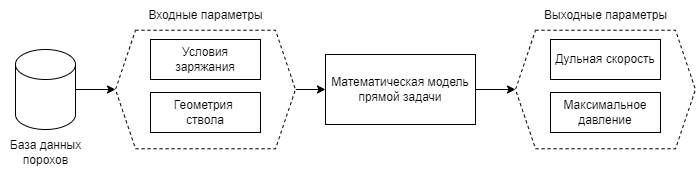
\includegraphics[width=0.7\textheight]{imgs/PZVB_sctruct.png}
\caption{Структура ПЗВБ}
\end{figure}

Имеется база данных порохов, а также математическая модель процесса выстрела. В случае данного варианта курсовой работы она является квазиодномерной. Формируются две группы входных параметров: геометрические и заряжания.
Первая группа представляет из себя набор значений калибра, приведенной длины камеры и длины ствола. Вторая группа представляет из себя марку пороха, его массу. Далее все эти данные подаются на вход мат.модели. В резульате расчёта прямой задачи 
на выходе получаем дульную скорость и максимальное давление (а также распределение этих параметров по координате в каждый момент времени).

Рассмотрим исходные данные для решения ОЗВБ. Заданным характеристикам $d$, $q$ и $v_{\text{pm}}$ соответствует бесконечное число вариантов геометрии ствола и параметров порохового заряда. Наборов таких параметров, соответствующим исходным данным, называют баллистическим решением (БР). Множество таких БР образуют бесконечное множество баллистических решений (МБР), обозначим это символом $\Theta$.

Решением обратной задачи внутренней баллистки является множество допустимых баллистических решений (МДБР) $\Omega$. Для того, чтобы его получить, т.е. выполнить преобразование вида $\Theta \longrightarrow \Omega $, необходимо наложить ограничения на $\Theta $. Те баллистичекие решения, которые будут удовлетворять этим ограничениям, образуют $\Omega $.

Определим набор данных для построяния МДБР. Характеристики порохового заряда (полный импульс $I_e$, геометрические тип и размеры порохового зерна) выбираются из вполне себе конечного, дискретного множества порохов, которое составляют базу данных порохов (БД). Структура БД порохов имеет вид $[\Pi_1, \Pi_2, \Pi_3,...,\Pi_N]$. Выбор конкретной марки $\Pi_i$ из этого множества подразумевает и выбор всех хараектристик порохового заряда. При выбранной марке порохового заряда баллистическое решение решение определяется только его массой $\omega$ и объёмом каморы $W_0$.
В таком случае в качестве независимых переменных удобно выбрать плотность заряжания $\varDelta$ и отношение массы снаряда к массе пороха $ \omega / q$.

Таким образом, решение прямой задачи, позволяющее отнести баллистическое решение к $\Omega $, можно представить в виде преобразования вводных данных из набора $[\varDelta,  \omega / q,  \Pi_i ]$
в требуемые выходные данные, например, максимального давления, длину ведущей части канала ствола и относительного положения снаряда во время сгорания пороха $\eta_{\text{ne}} = l_e / l_m$:

\begin{equation}
    [\varDelta, \omega / q,  \Pi_i] \longrightarrow [p_{\text{max}}, x_m, \eta_{\text{ne}}]
\end{equation}

Такой набор позволяет определить БР единственным образом. Также из данной совокупности входных и выходных данных можно составить любой критерий. Стоит отметить, что для смеси порохов структура данных примет иной вид:

\[
 [\varDelta, \omega_\Sigma / q,  \Pi_i, \Pi_j, \alpha_i] \longrightarrow [p_{\text{max}}, x_m, \eta_{\text{ne}}], 
\]
где $\omega_\Sigma = \omega_i + \omega_j$ -- суммарная масса порохового заряда, $\alpha_i = \omega_i / \omega_\Sigma $ -- массовая доля пороха марки i в общем заряде.

Далее на выходные данные накладываются ограничения. Все баллистические решения, прошедшие через данный «фильтр», образуют МБДР. В результате можно построить схему решения ОЗВБ на рисунке 2.2. 


\begin{figure}[h]
\centering
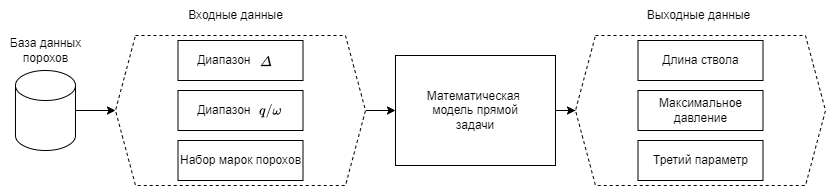
\includegraphics[width=0.65\textheight]{imgs/OZVB_STRUCT.png}
\caption{Структура ОЗВБ}
\end{figure}


\section{Методика решения обратной задачи внутренней баллистики}
Рассмотри методику решения обратной задачи внутренней баллистики. Её основну составляет многократное к прямой задаче в процессе перебора различных комбинаций параметров.
В целом, подход к решению предполгает: 

\begin{enumerate}
    \item  Задание диапазонов варьирования для  $\omega / q$, $\varDelta $ и марок порохов $\Pi$.
    \item  Диапазоны разбиваются сеткой (пример: функция np.linspace из пакета Numpy [6]).
    \item  Для каждой комбинации параметров  $\omega / q$, $\varDelta $ и  $\Pi_i$ производится решение прямой задачи.
    \item  Произодится проверка ограничений.
    \item  При выполнении ограничений баллистическое решение попадает в МДБР; в ином случае оно не рассматривается.
\end{enumerate}

Требования к курсовой работе заставляют также учитывать и пороховые смеси. В таком случае методика решения немного видоизменяется:

\begin{enumerate}
    \item  Задание диапазонов варьирования для  $\omega / q$, $\varDelta $ и марок порохов $\Pi$.
    \item  Диапазоны разбиваются сеткой (пример: функция np.linspace из пакета Numpy [6]).
    \item  Для каждой комбинации параметров  $\omega / q$, $\varDelta $, $\Pi_i$ и $\Pi_j$ производится решение прямой задачи.
    \item  Произодится проверка ограничений.
    \item  При выполнении ограничений баллистическое решение попадает в МДБР; в ином случае оно не рассматривается.
\end{enumerate}

В результате получаются некоторые области для каждой марки пороха, которые можно визуализировать на плоскости ($\varDelta, \omega / q $).
Смеси порохов, к сожалению, не поддаются такой простой визуализации. О решении этой проблемы будет идти речь в следующих пунктах.

\section{Предварительная оценка применимости различных марок порохов}

При решении ОЗВБ возникает потребность перебирать большое количество порохов для каждого выстрела, что неизменно влечёт за собой увеличение объема вычислений.

Пусть имеется абстрактная камора с зарядом пороха, имеющая 30 вариантов объема. Дискретизируем её так, чтобы она всегда разбивалсь на 5 равных частей. Также имеется набор из 102 порохов. Смесь состоит из двух порохов. Пороха не могут повторяться. На рисунке 2.3 представлена вспомогательная картинка.
Найдем число комбинаций: 

\[
 \Pi_1 \cdot \Pi_2 \cdot 30 \cdot (4+2) = 102 \cdot 101 \cdot 30 \cdot 6 = 1854360 \text{ комбинаций},
\]
где $\Pi_1, \Pi_2$ -- позиции порохов, (4+2) означает 4 варианта смеси и 2 варианта, когда камору заполняет только один порох.

\begin{figure}[h]
\centering
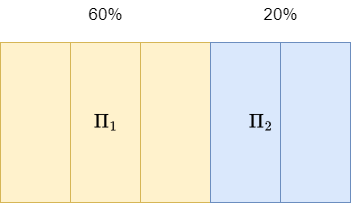
\includegraphics[width=0.5\textheight]{imgs/KAMORA.png}
\caption{Один из вариантов заполнения камеры}
\end{figure}

Проанализируем изменение числа комбинаций при условии, что пороховая смесь будет состоять из трёх и четырёх. На рисунке 2.4 представлена гистограмма зависимости количества комбианций от числа порохов в смеси.
Отсюда можно сделать вполне очевидный вывод, что при увеличении числа порохов в смеси растёт и объём вычислений, хотя можно и уточнить, что он увеличивается на (103-n), где n -- номер пороха в смеси, при условии, что пороха не могут повторяться. Без
этого условия объём расчётов увеличивается на количество добавленных марок пороха.

\begin{figure}[H]
\centering
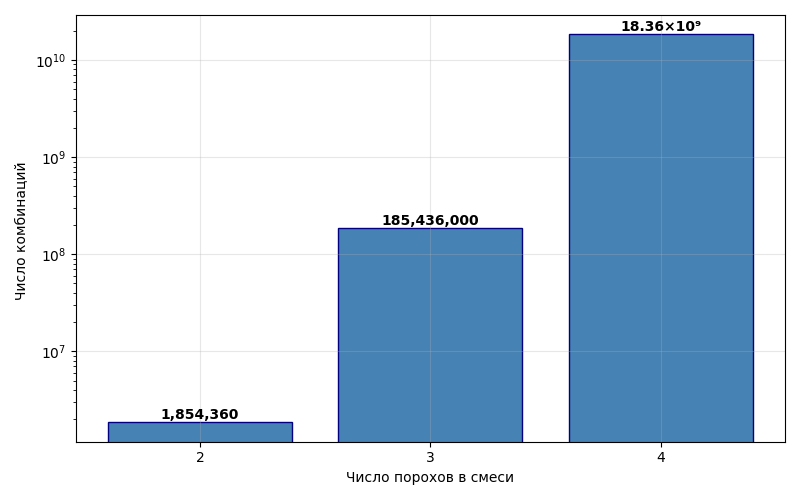
\includegraphics[width=0.5\textheight]{imgs/GISTO.png}
\caption{Число комбинаций порохов}
\end{figure}

Так как возможности ЭВМ не безграничны, и рано или поздно при включении такого перебора на несколько миллионов комбинаций компьютер уйдет в перезагрузку из-за недостатка оперативной памяти, то стоит предпринять усилия
для сокращения количества вычислений не уменьшая при этом точности расчёта. Это стоит начать с порохов: не стоит брать во внимание все марки.

Стоит начать с прототипа орудийной системы, лежащего в основе данного варианта курсовой работы. Этим прототипом является 85-мм дивизионная пушка (Д-44), показанная на рисунке 2.5.

\begin{figure}[H]
\centering
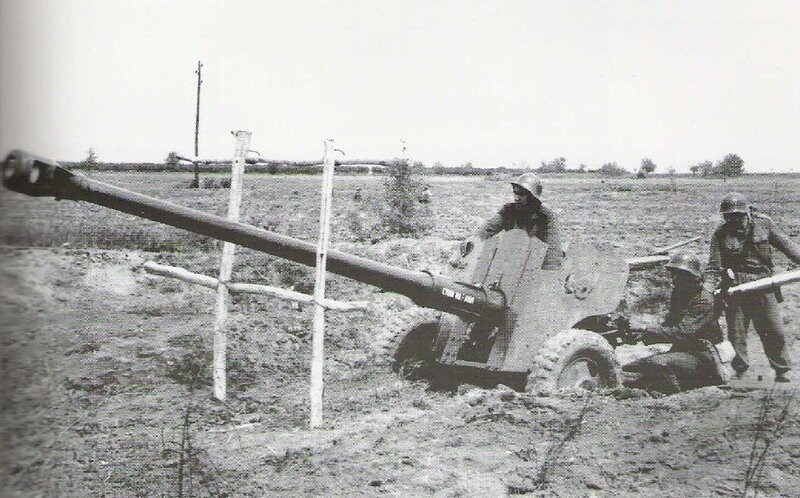
\includegraphics[width=0.35\textheight]{imgs/D44.jpg}
\caption{Пушка Д-44}
\end{figure}

Ниаболее близок к параметрам данного варианта курсовой работы бронебойный унитарный с подкалиберным снарядом катушечного типа 53-БР-365П

\begin{table}[h]
\centering
\caption{Характеристики бронебойного унитарного выстрела 53-БР-365П}
\begin{tabular}{|>{\raggedright\arraybackslash}p{0.4\textwidth}|>{\raggedright\arraybackslash}p{0.5\textwidth}|}
\hline
\textbf{Параметр} & \textbf{Значение} \\
\hline
Тип боеприпаса & Бронебойный унитарный выстрел с подкалиберным снарядом \\
\hline
Обозначение выстрела & 53-БР-365П \\
\hline
Масса выстрела & 11.42 кг \\
\hline
Масса снаряда & 5.0 кг \\
\hline
Масса заряда & 2.5—2.85 кг \\
\hline
Индекс ГРАУ & 54-Г-365 \\
\hline
Начальная скорость & 1050 м/с \\
\hline
Тип взрывателя & МД-8 \\
\hline
Масса пороха во взрывателе & ??? кг\\
\hline
\end{tabular}
\end{table}

Так как прототип арт.орудия -- дивизонная пушка сухопутных сил Д-44, то можно сделать вывод, что для неё нецелесообразно использовать пороха морской и береговой артиллерии, например 152/57. 
Таким образом, можно исключить из рассмотрения следующие пороха: 100/70, 180/57 ШЗ БП, 100/56, 180/57, 152/57 БП, 152/57 Ш, 130/50 Ш, 152/57, 180/57 БП, 180/60.



Пороха, главным образом, отличаются значениями полного импульса давления пороховых газов (далее импульс пороха) и значениями
коэффициентов формы зерна. Прочие характеристки менются незначительно и в первом приближении могут быть приняты некоторым средним значениям [3].

Зная массу снаряда $q$, требуемую дульную скорость $v_\text{pm}$ и калибр орудия, можно получить приближенное решение обратной задачи. В практическом плане 
такая приближенная оценка даст примерное значение полного импульса «условного» пороха. Полученное значение $I_e$ поможет сузить круг поиска подходящих под конкретную задачу порохов.
Формула значения импульса пороха: 

\begin{equation}
I_e = \frac{\sqrt{f \omega \varphi q B}}{S},
\end{equation}
где величина $\varphi$ определяется по формуле:

\begin{equation}
\varphi = \varphi_1 + \frac{1}{3q} \left( \omega_{\text{ign}} + \sum_{i=1}^{N} \omega_i \right).
\end{equation}
где $\omega_\text{ign}$ -- масса пороха воспламеняющего заряда, $\varphi_1 \thickapprox  1.02$.

Необходимая масса заряда может быть определена по следующей формуле: 

\begin{equation}
    \omega = \frac{\varphi_1 q}{\dfrac{2f}{(k-1)\ v^2_{pm}} \eta_{rm} - \frac{\zeta + 1}{3}},
\end{equation}
где $\zeta$ -- отношение масс воспламенительного и основного зарядов.

\begin{equation}
\zeta = \frac{P_{\mathrm{ign}}}{f} \left( \frac{1}{\Delta} - \frac{1}{\delta} \right) \frac{1}{1 + b p_{\mathrm{ign}} / f}
\end{equation}

\newpage
\begin{thebibliography}{9}
\bibitem{} \textbf{PyBallistics}
\bibitem{} \textbf{Matplotlib} 
\bibitem{} \textbf{Основная метода} 
\bibitem{} \textbf{МЕТОДЫ МАТЕМАТИЧЕСКОЙ ФИЗИКИ 
ДИФФЕРЕНЦИАЛЬНЫЕ УРАВНЕНИЯ 
С ЧАСТНЫМИ ПРОИЗВОДНЫМИ. 
ОСНОВНЫЕ ПОНЯТИЯ И КЛАССИФИКАЦИЯ } 
\bibitem{} \textbf{ЧИСЛЕННЫЕ МЕТОДЫ: ВВЕДЕНИЕ В ТЕОРИЮ РАЗНОСТНЫХ СХЕМ 2-е изд., испр. и доп. Учебник для вузов (Емельянов В. Н.)} 
\bibitem{} \textbf{Numpy}
\bibitem{} \textbf{Д44 пушка википедия}
\end{thebibliography}

\end{document}